\chapter{Background}
\label{Chapt2}
\section{Introduction}

This chapter will explore the fundamental information relevant to this project, with an emphasis on the world of DNS abuse and transparency. It will include a thorough investigation of the domain name system (DNS), its function in the online community, and the variety of abuses it faces. The history of widely used policies and organisations aimed at stopping DNS abuse, including a thorough examination of the DNS Abuse Institute and its achievements, is essential to our investigation. A 'competition landscape' providing a critical examination of current market choices, from automated solutions to human tactics, will be provided as we navigate through the current methodology and technology deployed to mitigate DNS abuse. The reader will obtain an in-depth understanding of the current situation of DNS abuse and the need for a more open, strong, and proactive strategy by analysing these various techniques and appreciating their strengths and weaknesses. This chapter emphasises the importance of the suggested solution in an era where digital authenticity is required, not only by providing information but also by laying the groundwork for its presentation as a better and essential progression in the battle against DNS abuse.

\section{Understanding DNS and Its Vulnerabilities}

The Domain Name System (DNS) is a significant part of the infrastructure of the Internet, serving as the key that converts computer-understandable IP addresses into human-friendly domain names. Although the DNS plays a vital role in maintaining ongoing online activities, privacy and security problems still arise. The ScienceDirect paper "Domain Name System Security and Privacy: A Contemporary Survey" provides a thorough analysis of these concerns which highlights the fundamental significance of the DNS while illuminating the weaknesses that malicious actors may take advantage of \cite*{sciencedirect2023dns}.

A variety of security threats exist, ranging from DNS infrastructure-targeting distributed denial of service (DDoS) assaults to cache poisoning and hijacking. Each of these attacks has the potential to do significant harm, including interruptions in service and the promotion of theft and spying. Due to the standard DNS design's lack of encryption, users' query data is vulnerable to abuse and eavesdropping, raising serious privacy problems. However, weaknesses do not mark the end of the story. In the same survey, new approaches are examined to improve DNS security and privacy. The use of DNSSEC (DNS Security Extensions), which authenticates DNS data and guarantees its integrity while repelling some types of attack, is one example of these advances in security measures. Moreover, privacy-enhancing technologies are being used to encrypt DNS queries, preventing eavesdropping and manipulation, such as DNS over HTTPS (DoH) and DNS over TLS (DoT). The environment of DNS threats and defences is always changing in sync with the internet. For systems to be robust and resilient, it is essential to understand these weaknesses and the continuous efforts being made to mitigate them. An in-depth discussion of DNS vulnerability details, the effects of these safety concerns, and creative solutions that aim to bring in a new era of DNS security and privacy will be provided in this section.

\section{Current efforts and organisations combatting DNS Abuse}

The DNS Abuse Institute, which will focus on DNS abuse to help in increasing safety and security through the domain name system, is going to be cantered on these efforts to address DNS abuse with a comprehensive approach throughout the infrastructure of the internet. It helps the internet community in the identification, reporting, and mitigation of DNS abuse in its mission to make the online environment more secure. Efforts by the institute, such as Compass Dashboards, provide vital data to registries and registrars that will enable proper decisions on combating DNS abuse. They prove the commitment towards transparency and education by issuing publications like the "DNSAI 2022 Annual Report" or "DNSAI Bulletin 2023 04; Account Takeovers," which provide insights regarding DNS abuse and how recommended mitigation practices \cite{dnsabuseinstitute2023}. Another such global strategy against DNS abuse has been contributed by the Internet Corporation for Assigned Names and Numbers (ICANN)\cite{icann2022dnsabuse}. In collaboration with the entire DNS community, ICANN supports a synchronised method in the development of policies and standards on how to mitigate DNS abuse while ensuring the openness and operability of the Internet. These participatory pillars hint at concerted efforts via policy development, technological developments, and stakeholder engagement as core in this collective approach towards combating DNS abuse \cite{dnsai2022report}. 



\section{Different Forms of DNS Abuse}

DNS abuse takes many forms, each with its procedures and effects on users and the internet as a whole. It is essential to understand these various pieces of evidence to create responses and regulations that work. This section will examine the comprehensive analysis of DNS abuse as presented, going into the description, mechanism, and impact of each kind.

\subsection{Phishing}
\begin{itemize}
    \item \textbf{Description:} Phishing is a technique aimed at deceiving individuals by creating website addresses that mimic those of companies, to trick users into revealing sensitive information such as login credentials, credit card numbers, or personal identification information \cite{webinarcare2023dnsstats}.
    \item \textbf{Mechanism:} This deception often occurs through emails or messaging services that direct users to websites resembling authentic ones \cite{jakobsson2006phishing}.
    \item \textbf{Impact:} Victims may suffer identity theft, financial fraud, and security compromise.
\end{itemize}

\subsection{Confusable Domains (Typosquatting)}
\begin{itemize}
    \item \textbf{Description:} Registering domain names that look visually similar to popular websites, taking advantage of typing errors or character similarities \cite{inta2023dnstypo}.
    \item \textbf{Mechanism:} Users may accidentally visit these websites when making a typo in a URL, potentially exposing them to malware or phishing attempts.
    \item \textbf{Impact:} Deception of users and potential harm to brand reputation \cite{edelman2008typosquatting}.
\end{itemize}

\subsection{Domain Hijacking}
\begin{itemize}
    \item \textbf{Description:} Unauthorised acquisition of domain names by exploiting security vulnerabilities in the domain registration system \cite{inta2023dnstypo}.
    \item \textbf{Mechanism:} Attackers may use tactics like social engineering, phishing, or exploiting security loopholes to gain control over a domain.
    \item \textbf{Impact:} Loss of website control, redirection to malicious sites, and potential data breaches.
\end{itemize}

\subsection{Botnets}
\begin{itemize}
    \item \textbf{Description:} Botnets involve controlling a group of computers infected with malware, used to carry out attacks or spread spam and malware \cite{citpyour}.
    \item \textbf{Mechanism:} Malware infects unsuspecting users’ computers, incorporating them into a network under the attacker's control.
    \item \textbf{Impact:} Can result in large-scale DDoS attacks, mass spam campaigns, and widespread malware dissemination.
\end{itemize}

\subsection{Fast Flux Hosting}
\begin{itemize}
    \item \textbf{Description:} A technique used to conceal the location of websites associated with phishing and malware distribution \cite{lin2013genetic}.
    \item \textbf{Mechanism:} Involves a network of compromised hosts that regularly modify DNS records to evade detection.
    \item \textbf{Impact:} Makes tracking and shutting down malicious sites difficult.
\end{itemize}

\subsection{Domain Generation Algorithms (DGA)}
\begin{itemize}
    \item \textbf{Description:} DGAs generate domain names that act as meeting points for botnets \cite{antonakakis2012throw}.
    \item \textbf{Mechanism:} Malicious software uses algorithms to generate a sequence of domain names for command-and-control servers.
    \item \textbf{Impact:} Adds complexity to efforts to disrupt botnet command and control channels.
\end{itemize}
\captionsetup{font= footnotesize}
\begin{figure}[H]
\centering
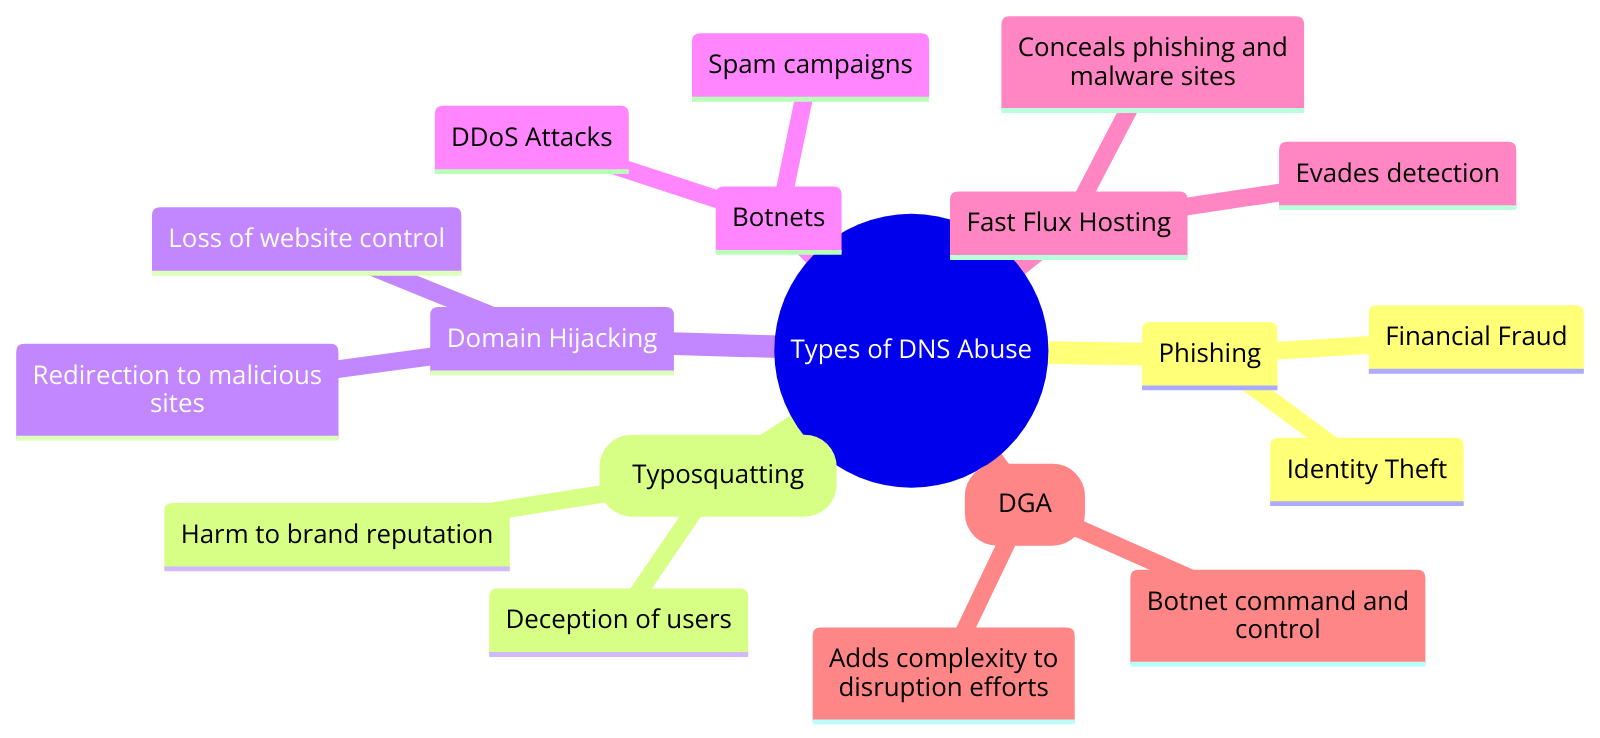
\includegraphics[width=1.0\textwidth]{background/DNSabuseForms.png}
\caption{Impact of DNS Abuse}
\label{fig:figureThree}
\end{figure}



\section{How DNS Abuse Harms Users}

DNS abuse has serious and detrimental effects for both users and organisations, going beyond basic technological disruptions. Identity theft is among the most direct and direct effects. Phishing attacks, a frequent type of DNS abuse, use realistic websites to trick visitors into revealing sensitive data. Such attacks can produce information that results in financial theft, unauthorised access to accounts, and long-term damage to a person's reputation and credit.

\subsection{Identity Theft}
\begin{itemize}
    \item \textbf{Phishing:} Phishing attacks often use domain names that imitate legitimate websites, fooling users into providing sensitive information such as usernames, passwords, or financial details, leading to potential identity theft \cite{godaddy2023dnsabuse, jakobsson2006phishing}.
\end{itemize}

\subsection{Financial Loss}
\begin{itemize}
    \item \textbf{Deceptive Transactions:} Users may be tricked into making payments to deceptive websites or unknowingly disclose their credit card information, resulting in financial losses \cite{godaddy2023dnsabuse, bohme2013economics}.
\end{itemize}

\subsection{Data Breach}
\begin{itemize}
    \item \textbf{Malware:} Malicious software spread through compromised DNS systems can allow unauthorized access to corporate data, leading to data breaches \cite{icann2022dnsabusetrends, fowler2016data}.
\end{itemize}

\subsection{System Compromise}
\begin{itemize}
    \item \textbf{Malware Infection:} Systems infected with malware due to DNS abuse can be exploited for further attacks, including the creation of botnets or the distribution of ransomware, resulting in system compromise \cite{dotmagazine2022dnsabuse, saxe2018malware}.
\end{itemize}
\captionsetup{font= footnotesize}
\begin{figure}[H]
\centering
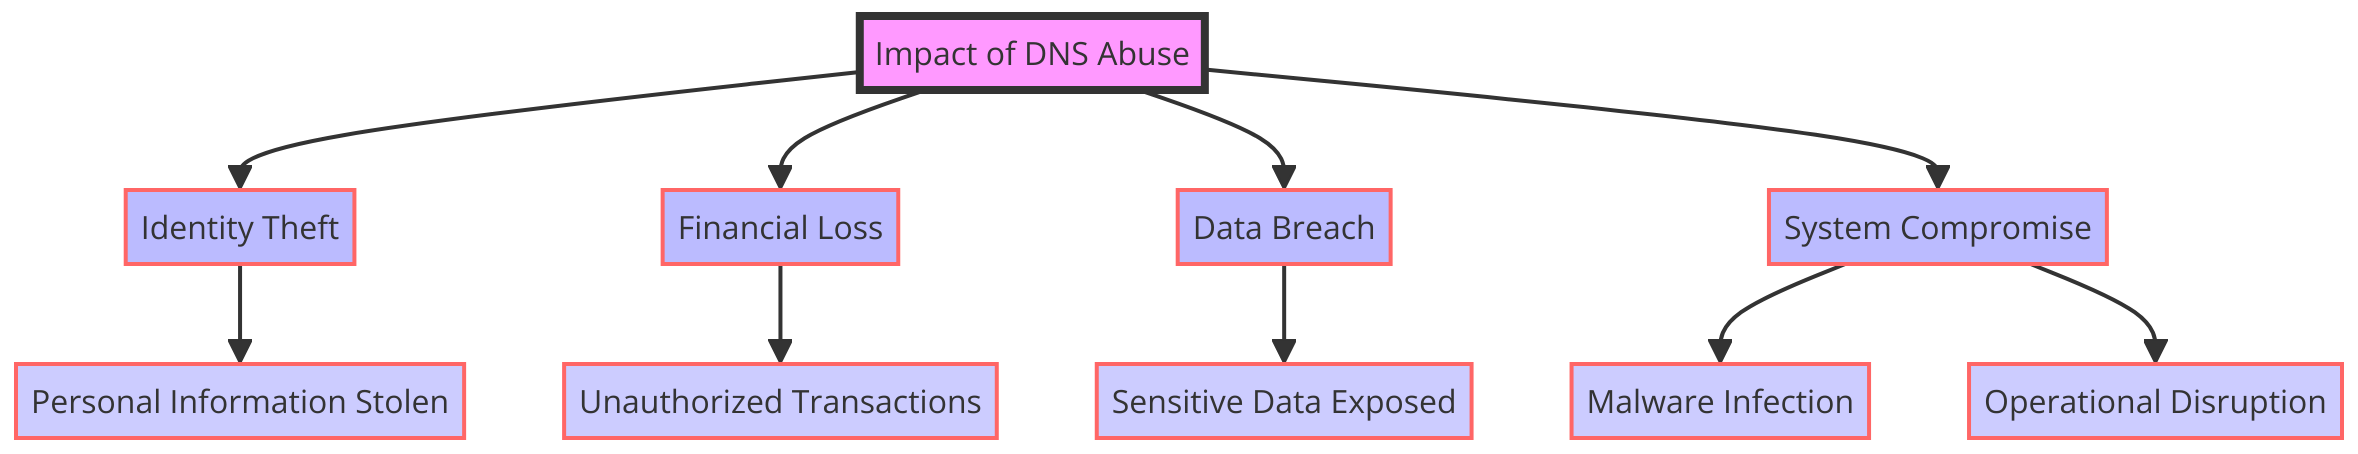
\includegraphics[width=1.0\textwidth]{background/DNSabuseHarm.png}
\caption{Different Forms of DNS Abuse}
\label{fig:figureFour}
\end{figure}


\section{Future Dangers of DNS Abuse}

As technology develops, so do cyber attackers' strategies and tools, creating a dynamic environment for DNS abuse that could present new risks in the future. The sophistication of attacks has increased, which is a major issue. Bad actors are always creating increasingly sophisticated methods to take advantage of DNS, such as creating more convincing phishing schemes and using advanced virus distribution networks.

\subsection{Increased Sophistication}
\begin{itemize}
    \item \textbf{Evolving Techniques:} Cyber attackers are constantly developing more sophisticated techniques to exploit DNS, such as advanced phishing schemes and malware distribution \cite{icann2022dnsabusetrends, wrightson2014advanced}.
\end{itemize}

\subsection{IoT Vulnerabilities}
\begin{itemize}
    \item \textbf{Expanding Vulnerabilities:} The widespread adoption of Internet of Things (IoT) devices, which often lack robust security measures, presents a growing target for DNS-based attacks \cite{circleid2020dnstrends, mahmoud2015internet}.
\end{itemize}

\subsection{Infrastructure Attacks}
\begin{itemize}
    \item \textbf{DNS as a Prime Target:} Attacks on DNS infrastructure can disrupt internet services on a large scale, including DDoS attacks targeting DNS providers or exploiting weaknesses in DNS protocols \cite{dotmagazine2022dnsabuse, dooley2017dns}.
\end{itemize}

\subsection{Deepfakes and AI}
\begin{itemize}
    \item \textbf{AI-Enhanced Phishing:} The use of AI technologies, such as deepfakes, has made phishing attacks more convincing and deceptive, manipulating audio and video content to impersonate trusted entities \cite{icann2022dnsabusetrends, schick2020deep}.
\end{itemize}

\subsection{Cloud Computing Vulnerabilities}
\begin{itemize}
    \item \textbf{Targeting Cloud Services:} As organisations increasingly rely on cloud-based services, bad actors are exploiting DNS vulnerabilities to attack these platforms, potentially leading to data breaches and service disruptions \cite{mather2009cloud}.
\end{itemize}

\subsection{Mobile Device Exploitation}
\begin{itemize}
    \item \textbf{Mobile DNS Attacks:} The rising usage of mobile devices has led bad actors to target smartphones and tablets through DNS-based attacks, which can lead to data theft and the spread of malware \cite{au2016mobile}.
\end{itemize}

\subsection{Cryptocurrency and Blockchain Exploitation}
\begin{itemize}
    \item \textbf{Crypto-Related DNS Attacks:} Attackers could exploit DNS vulnerabilities to redirect users to fake cryptocurrency exchanges or blockchain platforms, leading to financial fraud and theft of digital assets \cite{bashir2019advanced}.
\end{itemize}

\subsection{Political and Information Warfare}
\begin{itemize}
    \item \textbf{DNS in Cyber Warfare:} The manipulation of domain name systems can be used to spread misinformation or disrupt services during significant political events, serving as a tool for political and information warfare \cite{chapple2021cyberwarfare}.
\end{itemize}

\subsection{Exploiting Emerging Technologies}
\begin{itemize}
    \item \textbf{Abuse in New Tech Domains:} As new technologies such as 5G, AI, and quantum computing advance, tactics involving DNS abuse are likely to evolve, potentially leading to more sophisticated attacks \cite{brunner2021cybersecurity}.
\end{itemize}

\subsection{Supply Chain Attacks}
\begin{itemize}
    \item \textbf{DNS in Supply Chain Compromise:} DNS manipulation can also be employed as part of supply chain attacks, targeting software updates or cloud-based services to compromise organisations \cite{boyson2014cyber}.
\end{itemize}

By understanding these future dangers and emerging trends, stakeholders can better prepare and adapt their strategies to anticipate and counteract the evolving nature of DNS abuse.


\captionsetup{font= footnotesize}
\begin{figure}[H]
\centering
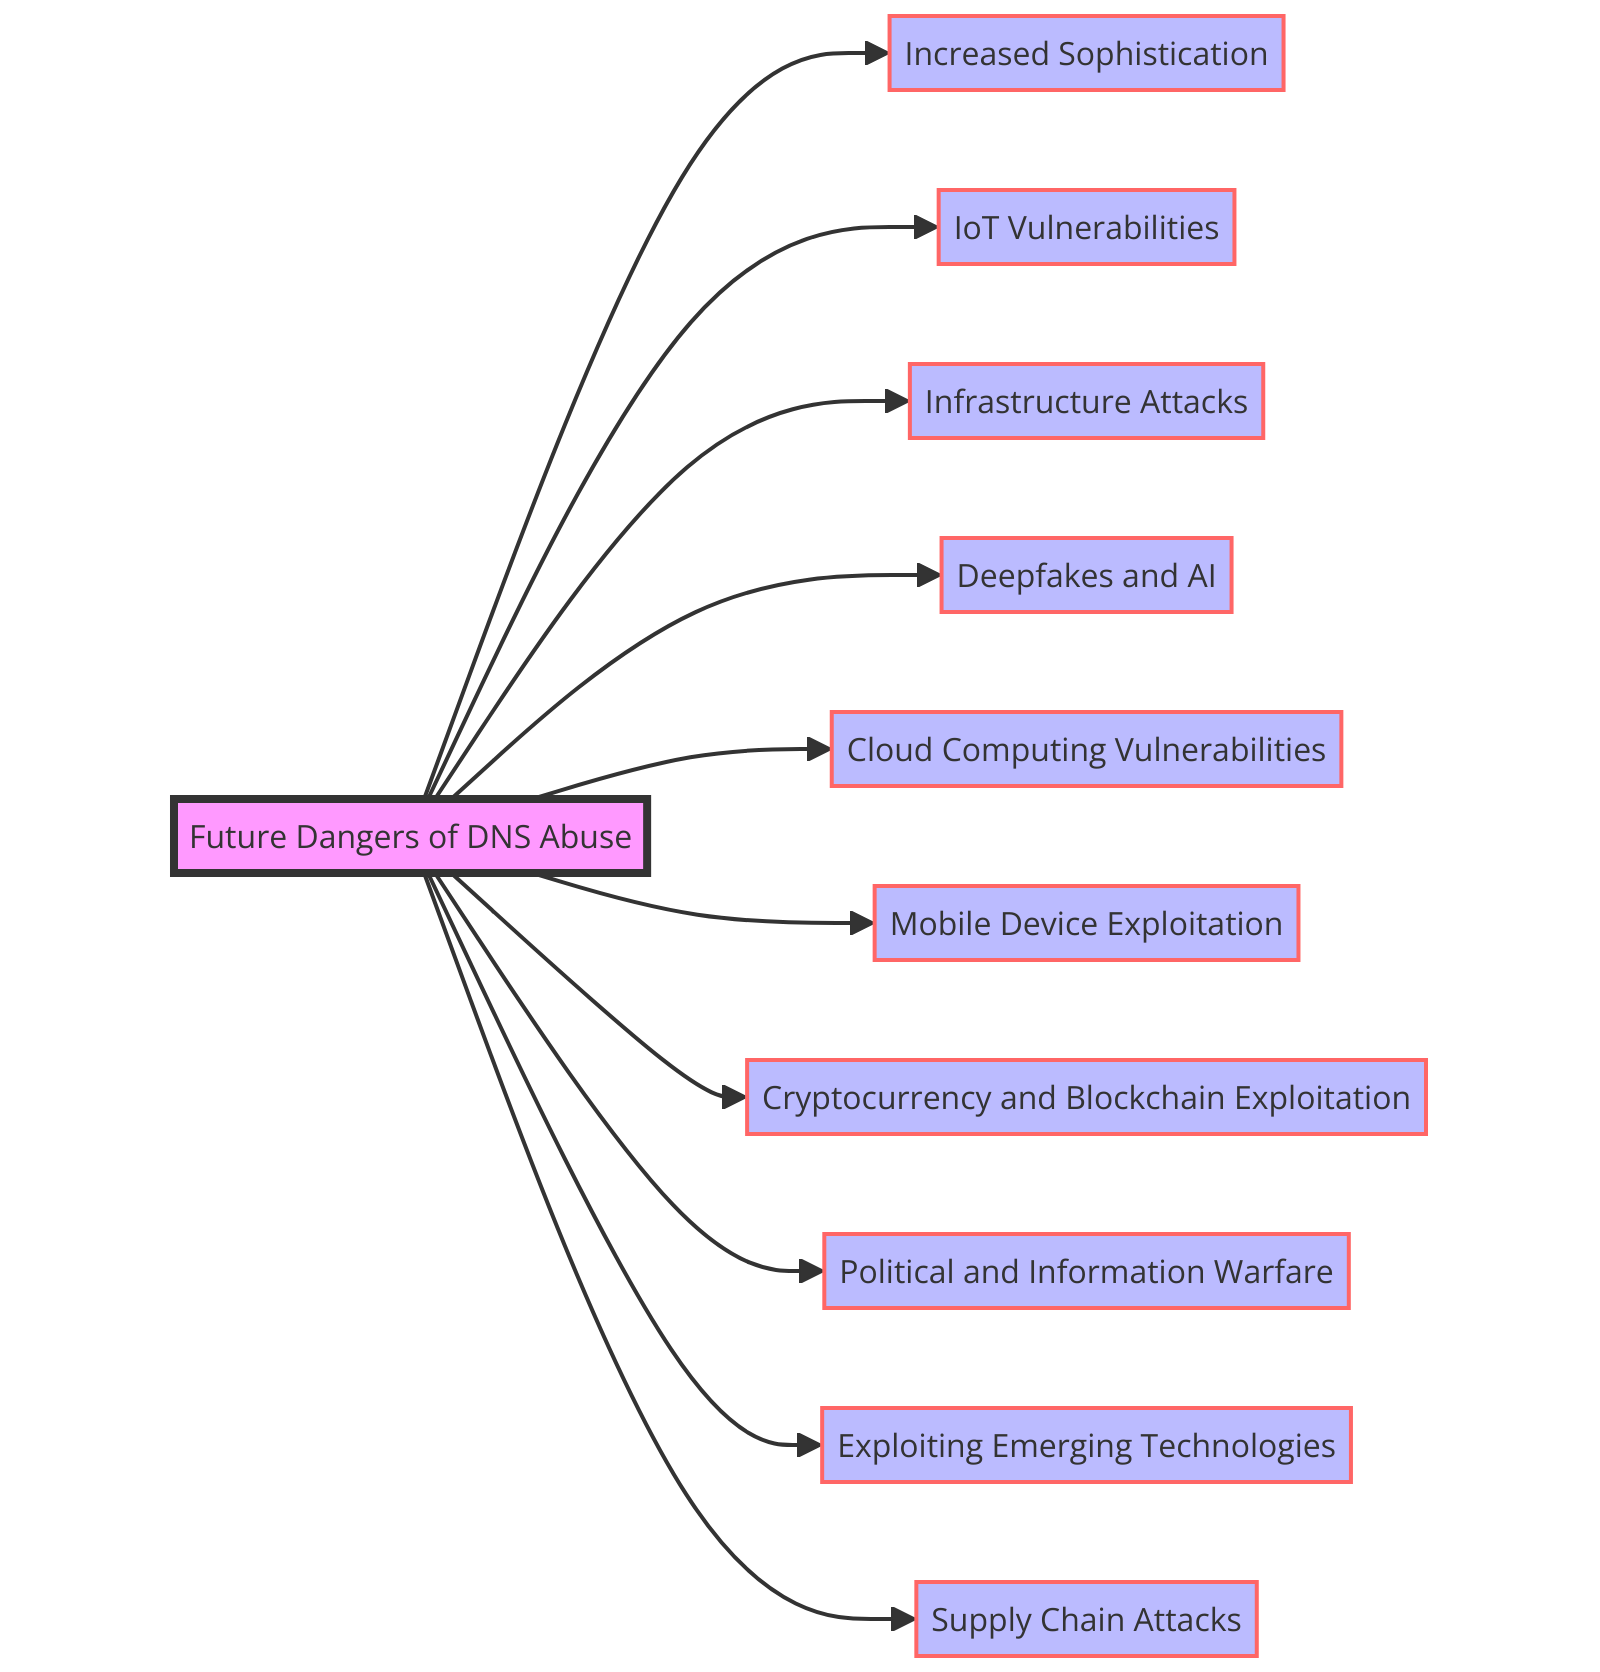
\includegraphics[width=1.2\textwidth]{background/DNSfutureDanger.png}
\caption{Future dangers of DNS abuse}
\label{fig:figureFive}
\end{figure}
\newpage


\section{Foundational Mitigation Strategies and Best Practices }

To address the broad nature of the threats, mitigating DNS abuse requires an integrated strategy that integrates multiple strategies and best practices. Setting up procedures for reporting and monitoring is one fundamental tactic. Automated systems have the ability to track domain name registration patterns that may indicate DNS abuse, and protocols for reporting questionable actions can help ensure prompt intervention \cite{icannndnssec}. To confirm security and ensure that systems have not been compromised, regular audits of DNS setups and domain registrations are also necessary \cite{lucas2021tls} .

\begin{enumerate}
    \item \textbf{Monitoring and Reporting}
    \begin{itemize}
        \item Implementation: Use automated systems to monitor the registration of domain names for patterns that may indicate DNS abuse \cite{icannndnssec}. Establish procedures for reporting activities to authorities or cybersecurity organisations \cite{lucas2021tls}.
    \end{itemize}
    \item \textbf{Security Awareness Training}
    \begin{itemize}
        \item Implementation: Develop training programs for users and IT staff with a focus on recognizing phishing attempts, practicing browsing habits, and understanding DNS security.
    \end{itemize}
    \item \textbf{DNS Security Extensions (DNSSEC)}
    \begin{itemize}
        \item Implementation: Deploy DNSSEC to ensure the integrity of DNS data. This involves signing DNS records to protect against modifications and DNS spoofing.
    \end{itemize}
    \item \textbf{Multi-Factor Authentication (MFA)}
    \begin{itemize}
        \item Implementation: Enforce multifactor authentication (MFA) for domain registrars and interfaces used to manage DNS \cite{icannndnssec}. This adds a layer of security beyond passwords, helping to prevent unauthorised domain transfers or alterations \cite{moghaddam2014ecco}.
    \end{itemize}
    \item \textbf{Blacklisting and Takedown Services}
    \begin{itemize}
        \item Implementation: Collaborate with cybersecurity firms to identify and blacklist domains engaged in malicious activities. Establish response teams dedicated to taking down domains involved in DNS abuse.
    \end{itemize}
    \item \textbf{Collaboration}
    \begin{itemize}
        \item Implementation: Foster collaboration among internet service providers (ISPs), domain registrars, governments, and cybersecurity organizations. Share intelligence and best practices to collectively enhance defense against DNS abuse \cite{skopik2017collaborative}.
    \end{itemize}
    \item \textbf{Regular Audits}
    \begin{itemize}
        \item Implementation: Conduct security audits of domain registrations and DNS configurations to verify their security and ensure they have not been compromised \cite{coronado2014auditing}.
    \end{itemize}
    \item \textbf{Machine Learning}
    \begin{itemize}
        \item Implementation: Using AI and machine learning algorithms to analyse patterns in DNS traffic and proactively predict instances of DNS abuse \cite{icannndnssec}. This proactive approach enables the identification of threats before they materialise \cite{tsukerman2019machine}.
    \end{itemize}
    \item \textbf{Geo-Blocking and IP Filtering}
    \begin{itemize}
        \item Implementation: Deploy geo-blocking and IP filtering techniques to limit access to DNS services from regions that have a history of DNS abuse. This can reduce the risk that attackers will use these services to carry out malicious activities or distribute malware \cite{meeseedited}.
    \end{itemize}
    \item \textbf{Enhanced Domain Validation Procedures}
    \begin{itemize}
        \item Implementation: Enhance the domain registration process by implementing validation procedures. This may involve verifying the identity of individuals or organizations that register domains, especially domains that resemble brands or fall into sensitive categories. By taking these measures, we can strengthen security and mitigate risks associated with fraudulent domain registrations.
    \end{itemize}
\end{enumerate}

Each of these strategies plays a role in creating a comprehensive defence against DNS abuse. By integrating these tactics, organisations can establish robust, proactive measures to detect, prevent, and mitigate the ever-evolving threats posed by DNS abuse.

\captionsetup{font= footnotesize}
\begin{figure}[H]
\centering
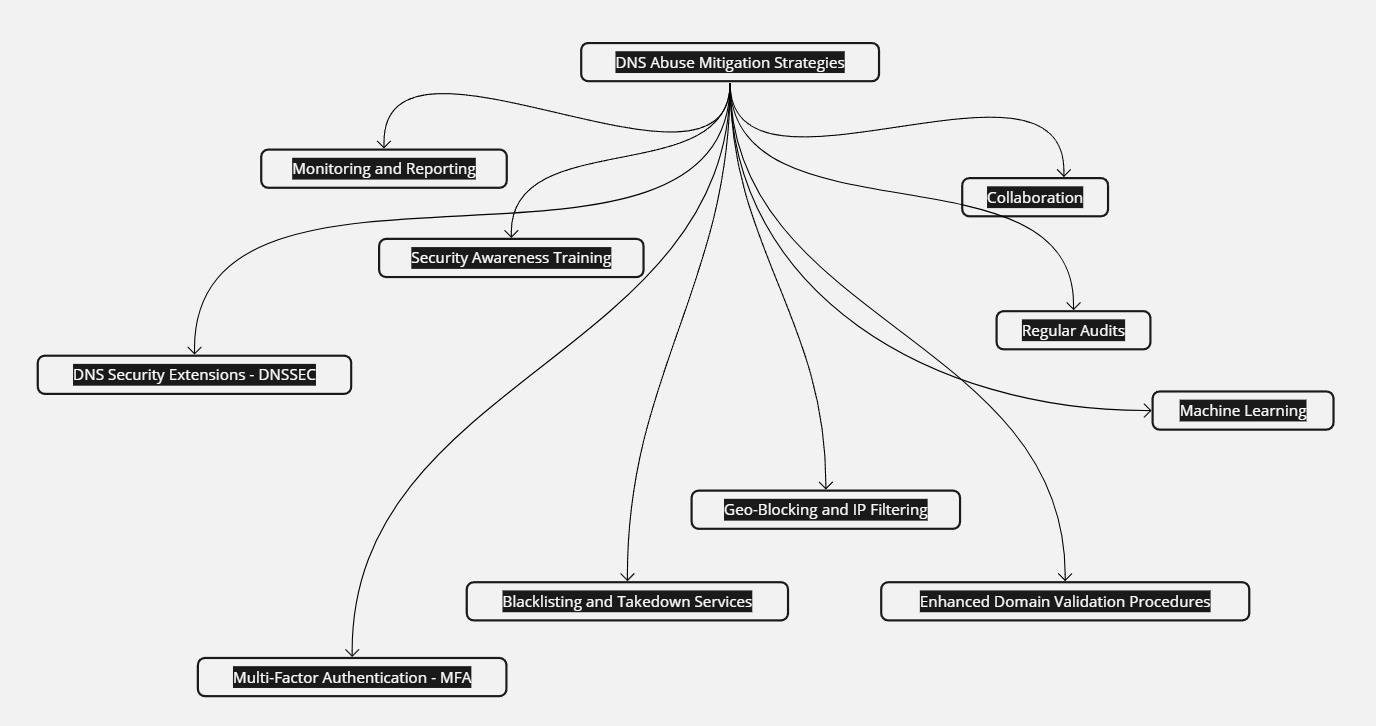
\includegraphics[width=0.7\textwidth]{background/DNSabuseMiti.jpg}
\caption{Future dangers of DNS abuse}
\label{fig:figureSix}
\end{figure}




\section{Summary and Synthesis}

After exploring the different forms of DNS abuse , How DNS abuse harms user , Future Dangers of DNS abuse and Mitigation Strategies and Best Practices. I have designed a table that has DNS abuses and the best possible mitigation strategies to help them against them, taking into account the transparency story behind it , user harm and reasoning. 

{
\footnotesize

\begin{longtable}{|p{2.5cm}|p{2.5cm}|p{4cm}|p{3cm}|p{4cm}|} 

\hline
\textbf{DNS Abuse } & \textbf{User Harm} & \textbf{Mitigation Strategy} & \textbf{Reasoning} & \textbf{Transparency Aspect} \\ \hline
\endfirsthead

\multicolumn{5}{c}%
{
\hline \textbf{DNS Abuse} & \textbf{User Harm} & \textbf{Mitigation Strategy} & \textbf{Reasoning} & \textbf{Transparency Aspect} \\ \hline
\endhead

\hline \multicolumn{5}{|r|}{{Continued on next page}} \\ \hline
\endfoot

\hline
\endlastfoot
Phishing & \mbox{Identity Theft}, Financial Loss &  \mbox{Security Awareness} \mbox{Training, Enhanced Domain} Validation Procedures & \mbox{Training helps users} \mbox{recognize phishing} \mbox{attempts. Validation} prevents registration of mimic domains. & \mbox{Increases awareness and} \mbox{scrutiny during domain} registration. \\ \hline

\mbox{Confusable} Domains \mbox{(Typosquatting)} & Unauthorised Account Access & \mbox{Enhanced Domain} \mbox{Validation Procedures}, Regular Audits & \mbox{Prevents Registration} of Similar Domains. \mbox{Audits ensure} \mbox{compliance.} & \mbox{transparent domain} \mbox{registration process.} \\ \hline

\mbox{Domain} \mbox{Hijacking} & \mbox{System} \mbox{Compromise}, \mbox{Data Breach} & \mbox{Multi-Factor Authentication} (MFA), Regular Audits & \mbox{MFA secures domain} management. \mbox{Audits verify security} measures. & \mbox{Accountability in domain} management. \\ \hline

Botnets & \mbox{Malware} \mbox{Distribution} & Collaboration,Machine Learning & \mbox{Intelligence Sharing} \mbox{identifies botnet} \mbox{activities. AI predicts} \mbox{the formation of} \mbox{botnets}. & \mbox{Shared responsibility and} proactive detection. \\ \hline

\mbox{Fast Flux} \mbox{Hosting} & \mbox{System Infections} & Blacklisting and Takedown Services, Geo-Blocking & \mbox{Rapid response to} \mbox{malicious domains.} Restrict access from risky regions. & Responsive and transparent threat management. \\ \hline

\mbox{Domain} \mbox{Generation} Algorithms (DGA) & \mbox{Malware} \mbox{Distribution} & \mbox{Machine Learning, DNS} \mbox{Security Extensions} (DNSSEC) & AI detects abnormal \mbox{patterns. DNSSEC} \mbox{prevents spoofing.} & Integrity and trust in DNS data. \\ \hline

\mbox{IoT} \mbox{Vulnerabilities} & \mbox{Unauthorised} \mbox{Access, Data} \mbox{Breach} & \mbox{Security Awareness} \mbox{Training, Collaboration} & \mbox{Educates on security} \mbox{practices.} \mbox{Collaboration on best} \mbox{practices.} & \mbox{Open exchange of} \mbox{knowledge and efforts.} \\ \hline

Infrastructure Attacks & \mbox{DDoS Attacks}, \mbox{System Downtime} & DNSSEC, Collaboration & Protects DNS data integrity. Sharing of threat intelligence. & \mbox{Collective action}  \mbox{strengthens the DNS} infrastructure.  \\ \hline

Deepfakes and AI & \mbox{Identity Theft}, \mbox{Misinformation} & \mbox{Security Awareness} \mbox{Training, Monitoring} & \mbox{Recognising Phishing.} \mbox{Monitor} \mbox{AI threats.} & \mbox{Vigilance and prompt} \mbox{threat reporting.} \\  \hline

\mbox{Cloud} \mbox{Computing} Vulnerabilities & \mbox{Data Breach}, \mbox{Unauthorised} Access & Regular Audits, Enhanced Validation & \mbox{Secure DNS settings} \mbox{in cloud services.} \mbox{Prevents exploitation.} & \mbox{Framework for secure} \mbox{domain use in cloud.} \hline

\mbox{Mobile Device} Exploitation & Unauthorised Access, Financial Loss & \mbox{MFA, Security Awareness} Training & \mbox{Secures account} \mbox{access.} \mbox{ Raises awareness} of threats. & Mobile security awareness and protection. \\ \hline

\mbox{Cryptocurrency} \mbox{and Blockchain} Exploitation & \mbox{Financial Theft}, \mbox{Account} \mbox{Compromise} & \mbox{Enhanced Validation}, \mbox{Collaboration} & \mbox{Prevents fraudulent} \mbox{domain registrations.} \mbox{Collaboration on} \mbox{threat intelligence.} & Security registration and defence of domains. \\ \hline

\mbox{Political and} Information Warfare & Misinformation, Political \mbox{Manipulation} & Monitoring, Collaboration & \mbox{Monitoring abuse in} \mbox{campaigns. Unified} \mbox{response to } \mbox{misinformation.} & Transparency in monitoring and collective action. \\ \hline

\mbox{Exploiting} Emerging \mbox{Technologies} & System \mbox{Vulnerabilities} &\mbox{ Machine Learning,} \mbox{Collaboration} & \mbox{Analytics to predict} \mbox{DNS abuse. Share} \mbox{knowledge about} \mbox{threats.} & \mbox{Innovation in defense}  \mbox{strategies and sharing.} \\ \hline

\mbox{Supply Chain} \mbox{Attacks} & \mbox{System} \mbox{Compromise,} Data Breach & Regular Audits, Blacklisting & \mbox{Audits for DNS} \mbox{integrity. Rapid} \mbox{response to threats.} & \mbox{Transparency in supply} \mbox{chain security.} \\ \hline

\caption{Mitigation Strategies Against DNS Abuse and Their Impact on Users} 

\end{longtable}

}

Finally , This chapter has examined all aspects of DNS abuse,  the various forms, the serious harm it does, as well as potential future threats and new trends. To create efficient regulations and countermeasures, it is essential to understand the extent and consequences of DNS abuse. The conversation emphasised DNS's vital function in the digital ecosystem as well as its susceptibility to abuse. Significant progress towards resolving these issues has been made by organisations like the DNS Abuse Institute and ICANN, as well as developments in DNS privacy and security technologies like DoT and DoH. However, as new technologies are incorporated into the equation and the threat environment changes in sophistication, it becomes increasingly important to adopt alert, flexible, and cooperative strategies.  

The mitigation techniques and best practices discussed in this chapter provide a roadmap for mitigating DNS abuse. Every tactic contributes to a defence mechanism, from advanced technology solutions and improved methods for validation to monitoring and reporting. It is impossible to overestimate the value of cooperation, regular checks, and the application of cutting-edge technologies to anticipate and mitigate DNS abuse. After analysing the data, it is evident that a team effort is needed to comprehend, track, and mitigate DNS abuse. A complex strategy that integrates multiple techniques and encourages collaboration across industries is required instead of a single, insufficient strategy. Our approaches to preserving the integrity and security of the DNS and, consequently, the larger internet infrastructure must adapt as does the digital environment.

By understanding the connections between different aspects of DNS abuse and reinforcing the collective effort required for effective mitigation, stakeholders can be better prepared to face the challenges ahead. This chapter sets the stage for further research and action, with the aim of contributing to a safer and more secure digital world.



\chapter{State of the Art}

This chapter explores the strategies being employed to mitigate DNS abuse as well as new developments in this field. Explores and evaluates the effectiveness and transparency of multiple mitigation techniques, including DNS filtering and threat intelligence in which information about cyber attacks that experts organise and analyse. Additionally, the use of domain-generating techniques and DoT and DoH are two novel forms of DNS abuse that are highlighted in this section. Along with the role of AI and machine learning in identifying and mitigating DNS abuse is covered. The final half of the section includes a discussion on potential future research areas and technologies to improve DNS abuse mitigation. Case studies offer practical insights into DNS abuse occurrences. 


\section{Current Strategies and Their Effectiveness in Relation to DNS Abuse}


DNS abuse presents a significant challenge for internet entities involved in domain name management. Various approaches are employed to mitigate such abuse, including DNS filtering, which regulates access to specific websites and prevents you from accessing malicious sites that can administer phishing and ransomware. Additionally, threat intelligence methodologies leverage data analysis to identify potential risks, as exemplified by \cite{schmid2021thirty}. Anomaly detection plays a role in identifying suspicious DNS activities indicative of malicious intent using Packet Analysis to analyse individual packets for DNS allowing for real-time detection and statistical analysis, which involves performing statistical analysis on a large dataset of DNS traffic. However, these methods can encounter operational challenges, such as errors and the need for fast access to critical threat data. 

\subsection{Transparency in DNS Abuse Mitigation: A Case Study of Cloudflare's Approach.}

Cloudflare is firmly committed to transparency \cite{cloudflare_transparency_2022}, the cornerstone of its relation with customers, guiding its approach to DNS abuse reports and requests that may come from law enforcement. This shaves their actions and policies to mold a trustworthy environment while addressing internet safety and privacy concerns. Their approach to handling DNS abuse reports and law enforcement requests is grounded in three core principles:

\begin{enumerate}
    \item Require Due Process:  Whatever shall be lawfully requiring due process of law enforcement and Cloudflare shall adhere in letter and spirit. They are neutral in behavior and do not intend to either hinder or facilitate law enforcement efforts more than necessary by law.
    \item Respect Privacy:  At Cloudflare, privacy is very important. They assure customers that anything of personal nature shared by them remains private and protected. The company makes a commitment not to sell, rent, or give out personal information without specific and unambiguous consent from the individual, applying this policy in both commercial and government or law enforcement requests.
    \item Provide Notice: Per the CloudFlare policy, they undertake to provide notice to any of their customers in case a subpoena or other legal process issues for customer or billing information relating to the use of its network, unless otherwise such disclosure is otherwise not permitted by law. This is aimed at making sure that 
    individuals and organizations are made aware before theirs can be given out.
\end{enumerate}

The Cloudflare Transparency Report for the latter half of 2022 gives deep statistics and trends based on DNS abuse reports over Cloudflare's response. It highlights:

\begin{enumerate}
    \item Abuse Reports: Cloudflare avidly responds to various abuse reports, and it has shown an enthusiastic commitment to maintaining a clean and lawful network. Some types of abuses reported include phishing, malware, content that violates copyright laws, among others.
    \item Actions Taken: Cloudflare not only reserves the right to review, accept or decline clients, but also ensures decisive actions against reported abuses by terminating hosting services from the domains taking part in technical abuses, such as phishing or any malicious activities. Such terminations are not limited to actions taken by content-based abuse and are handled differently.
    \item Termination of Services: Cloudflare suspends services to domains that do not take action to remedy reported instances of CSAM (Child Sexual Abuse Material) or are otherwise dedicated to distributing such material. Last year, in just the second half of 2022, alone, Cloudflare suspended service for 206 accounts and 530 domains connected to CSAM.
    \item IPFS and Ethereum Gateways: If a valid abuse report is received in regard to copyright, technical sanctions compliance, or otherwise, Cloudflare reserves the ability to disable access through its operated gateways to content on IPFS and the Ethereum network. 99 actions were taken on Ethereum gateways, and 1142 for IPFS during the second half of 2022.
    \item UDRP Requests: 21 UDRP (Uniform Domain-Name Dispute-Resolution Policy) responses resulted from verification requests to Cloudflare by an ICANN-approved dispute board in the second half of 2022, further illustrating its commitment to response in such legitimate concerns regarding domain name disputes.
    
\end{enumerate}

In addition , Cloudflare's careful description of compliance and due process with respect to handling law enforcement requests comes from their latest Transparency Report.
Below is a summary of the major areas covered.

\begin{enumerate}
    \item Legal Sufficiency Review: Each request is reviewed by Cloudflare for legal sufficiency before it is processed. This may range from ensuring compliance with necessary processes to all that is practically feasible within the purview of law to meet the need. They respect and safeguard the privacy of users and provide customer information to written requests from law enforcement that are validly issued based upon laws with valid legal process such as a subpoena or court order.

 \item Respect to International Privacy Laws: Cloudflare recognizes the potential conflict of privacy laws of different countries and when they receive requests from government, they legally challenge any request for data that is conflicting with the privacy laws of the country where the user stays.

 \item Emergency Disclosure Requests : Cloudflare takes very seriously all emergency disclosure requests. They may therefore make such disclosures to law enforcement without legal process when there appears to be an imminent danger of death or serious physical injury, and requests that law enforcement obtain legal process when time permits, therefore ensuring that the use of emergency disclosures remains a carefully controlled exception.

 \item  National Security Requests and Non-Disclosure Obligations: Cloudflare has made a lot of effort to challenge FISA court orders or National Security Letters (NSLs) in case they feel that the company received one with which their desire for transparency or releasing transparency reports cannot be met. In this regard, there was a period when the company fought legal prohibitions to report the receipt of NSLs, indicating its attitude of fighting for transparency and user privacy.

 \item  International Requests for Data: In the case of requests emanating from governments outside the United States, Cloudflare again evaluates them with strict adherence. The company responds to requests issued through U.S. courts by way of diplomatic processes like mutual legal assistance treaties (MLATs) and evaluates other international requests on a case-by-case basis. These include an analysis of local law, the request's compliance with international norms, and company policy.

 \item  Challenging Overly Broad or Inappropriate Requests: Over time, Cloudflare has long stated that it will challenge any law enforcement requests that are overbroad or issued wrongly and that act as an obstacle to their transparency with users. ., provided that due process of law requirements are met or that the exercise is intended to protect user rights in any request they may receive in or outside the USA.
\end{enumerate}

Public reporting by Cloudflare and working closely with law enforcement, as well as other partners, form important elements in its strategy of mitigating DNS abuse such as: 

\begin{enumerate}

\item Reporting to the Public and Transparency: Cloudflare keeps a high level of transparency in its reporting with regard to the types and volumes of abuse reports it receives and the measures which are put in place. This supports creating trust among clients and partners, evidencing action in fighting against abuse.

\item Law Enforcement Cooperation: The report shows how Cloudflare interacts and cooperates with many law enforcement agencies in the most approachable manner and without touching upon user privacy. It enables careful consideration of such a request for any action to be said legally justified and by so doing contributes to general mitigation efforts of DNS abuse.

\item Mitigation Actions: Cloudflare has taken affirmative action against DNS abuse. These actions include, but are not limited to, terminating such services when knowing of domains being used for phishing, distributing malware, and performing other activities that would harm a greater world. Termination of the access is done on content at the many different access points provided by Cloudflare, including any relating to abuse reports and, indeed, including IPFS and Ethereum gateways. This proves that the company is serious about mitigating DNS abuse.

\item Challenges to Preventing DNS Abuse: While Cloudflare does provide these tools, the report still refers to challenges that come with abuse mitigation. The struggle for balance between protection and abuse of free expression, legal and technical challenges when reacting to abuse reports, and from what kind of cooperation between key shareholders are, it is underlined, ongoing challenges.

\item Efficiency of Efforts to Mitigate DNS Abuse: Cloudflare transparency practices, through half-yearly publishing of transparency reports, lend a hand in acquiring insights into the mitigation of DNS abuse. This clearly shows their commitment and forward-leaning policy to minimize problems related to DNS abuse. However, their efficacy also depends on the broader ecosystem's capacity to solve the initial cause of this DNS abuse—an undiversified market where most other options for hosting are very limited.

\end{enumerate}

Some of the challenges with which Cloudflare is confronted in its transparency efforts and in mitigating DNS abuse are mentioned in the Transparency Report . They include such matters as the complexity of DNS abuse, keeping the fine balance between transparency and privacy, legal/regulatory compliance, and limitations of technical ability in mitigating the misuse while keeping the fine line. With these insights in mind, the following are recommendations that Cloudflare could use to identify potential enhancements in its processes:

\begin{enumerate}
    \item Enhanced Cooperation with Stakeholders: Cloudflare will enhance cooperation with law enforcement, other service providers, and international organizations to exchange views on best practices and come up with standard operational procedures on how exactly they will address DNS abuse. Joint efforts reduce identification time and intensify the ability to mitigate abuse throughout the whole of the internet ecosystem.
    \item Improve Abuse Detection Systems: Continuous investment in the best technologies and machine learning algorithms will better abuse detection and further its ability to respond to DNS abuse. Better detection will be less time-consuming in identifying and bringing down abusive content, therefore improving the entire internet safety concern as a whole.
    \item Transparency Reporting Enhanced: The reports on transparency from Cloudflare are simple to understand, yet they need more details about the identification of types of abuses faced by the domain name system and evaluate the process with respect to checking its effectiveness on all counts for mitigation. It will keep stakeholders up to date in providing much greater details when it comes to trend and pattern assessment in regard to the abuse, which will lead them in the process to fine-tune the directions of best practices for abuse mitigation.
    \item Better User Education and Awareness: Cloudflare would be in a position to prepare more materials and programs that educate its users about cybersecurity and the risks of abuse from DNS, and what they should do for protection. Enhanced user engagement on these can help build an enhanced internet environment.
    \item Advocate Policy and Legal Reforms: Cloudflare can do more in trying to advocate for policies that will potentially be challenged at various legal jurisdictions and cause potential conflict of privacy laws against law enforcement requests. Such a push for already formulated laws and put-in-place policies to balance user privacy against those interests supporting efforts in fighting DNS abuse, an improved offer may be realized. This policy helps offer protection against the abuse or even support for more coherent and efficient internet governance.
    \item Create a Multi-stakeholder Feedback Mechanism: A mechanism can be framed that ensures feedback from users, the civil society, and other stakeholders that would indicate how far Cloudflare has been successful in its transparency efforts and reducing abuse. Such suggestions thus received can then guide any subsequent policy revisions or enhancement of organizational policy.
    \item Continue to Challenge Overbroad Requests:  Cloudflare's willingness to continue fighting even with overbroad or inappropriate requests for user data in place remains praiseworthy. The possibility of being able to further prioritize the user and due process amongst this sort of situation implies some more badge of trust and a role model for the industry.
    
\end{enumerate}

\subsection{Advanced Mitigation Strategies}

Different methods are employed to mitigate DNS abuse, including the implementation of tools for blocking, awareness of potential threats, and identification of anomalous behaviour. DNS filtering entails the regulation of website access based on predetermined rules, which can have varied outcomes depending on the context in which can happen in different environments such as register and registry in which it implements mechanisms to compare DNS names to the block list and given set of rules then take the necessary action such as homographs attacks in which DNS filtering mechanism play a role in mitigating them by comparing domain names against block-lists and predefined rule to identify potentially malicious homographs as stated earlier. Threat intelligence plays a role in identifying potential dangers and detecting unusual activities within the DNS, as noted \cite{rizvi2022application}, such as allowing the proactive identification and assessment of potential threats and malicious activities which includes detecting patterns indicative of phishing, domain hijacking, malware distribution, and other forms of DNS abuse. Evaluating the effectiveness of these methods requires careful consideration of their performance in real-world scenarios. For instance, while DNS filtering can effectively block malicious content, it may inadvertently permit harmful elements to bypass the filtering process, potentially impacting user experience. Similarly, the efficacy of threat intelligence relies on the timeliness and accuracy of the data utilised. However, identifying anomalous behaviour poses challenges, as distinguishing between malicious actions and legitimate activities performed in innovative ways can be challenging.


\section{Emerging Trends in DNS Abuse}

The trends in DNS abuse had declined among some categories, such as botnets, malware, phishing, and spam. Much of this decline could be attributed to the multi-pronged approaches that ICANN itself launched around data analysis, community tools, and enforcement of registry and registrar obligations \cite{icann_dns_security_threat}. While continuing to be slow, adopting organisations did so under the compulsion of situations that left them no choice but to use the technology or by those for whom TLS adoption was a matter of technological innovation, choice, or desire for the embrace of technologies simpler and more robust from misdirection \cite{circleid_dns_trends_future}. One of the major issues has continued to be privacy, due to the fact that DNS queries have been accidentally found to give away user behaviors. One such move to enhance user privacy is the Query Name Minimization. The main concern has been how to remain vigilant against DNS abuses while improving privacy without impairing service efficiency.

\subsection{Evolving New Forms of DNS Abuse}

The field of cybersecurity is rapidly advancing, bringing forth new challenges as it evolves, and constantly moving the goalposts for defence mechanisms. The introduction of DNS over TLS (DoT) and DNS over HTTPS (DoH) is like a double-edged sword. Although these encryption protocols were designed to enhance privacy and security by encrypting DNS queries, they unintentionally provide attackers with means to disguise malicious traffic. This expands the attack surface, affecting everything from individual devices to corporate networks. For instance, attackers could leverage DoT and DoH in enterprise settings to avoid outdated security controls and establish hidden communication channels. Furthermore, Domain Generation Algorithms (DGAs) play an important role in cyber threats by automatically generating a large number of random domain names, making it extremely difficult to identify and shut down malicious sites. \cite{kaur2023artificial}. This tactic, integral to botnet command and control (C2) operations, significantly complicates cybersecurity defence efforts to predict and mitigate threats.

The adoption of DoT and DoH offers several benefits, such as enhanced privacy by preventing the surveillance of DNS queries and improved security through the encryption of DNS traffic, which weaken hackers' attempts to intercept or manipulate data. However, these protocols also allow attackers to hide their malicious activities, which poses challenges for traditional DNS security systems in detecting and filtering harmful content. Furthermore, these protocols might accidentally bypass content filtering policies, leading to potential security breaches within organisations.
Conversely, DGAs provide attackers with a method to evade detection and maintain C2 communications, as the dynamically generated domains are difficult to predict and pre-emptively block. This results in an overwhelming number of domain names for security mechanisms to monitor, complicating the threat intelligence process and necessitating continuous vigilance and blacklist updates. The widespread adoption of these technologies underscores the need for cybersecurity professionals to adopt a proactive and informed stance, understanding their potential for exploitation and developing comprehensive strategies. These strategies must strike a balance between the benefits of encryption and domain generation and the imperative to prevent DNS abuse, ensuring the integrity and security of the online environment.


\subsection{Predictive Measures and Their Transparency}

Efforts to mitigate DNS abuse are set toward immediately slowing such activities by utilising complex systems and advanced machine learning algorithms to detect patterns indicative of DNS abuse. Articulating and sharing insights about the decision-making processes in predictive modelling is considered significant as well as the efforts by registrars and registries, acting together, in the context of DNS Abuse Transparency are comprehensive. These entities will invoke a wide range of mitigation measures to minimise the damage and losses related to the DNS, which will ensure the development of a more secure and trusted Internet environment. Some key mitigation strategies are account-based remediation in the way that accounts which are maliciously generated are locked out and further validated, in addition to monitoring third-party feeds and reports from cybersecurity organisations, law enforcement, and the public to discover and address abuse early. Moreover, this mitigation involves malware analysis, which comes from attacks to the communication infrastructure and the corresponding IP addresses, through either suppression or sinkholing in the context of botnets and the use of Domain Generation Algorithms (DGAs) that direct botnet traffic \cite{ M3AAWG2024}. Most specifically, sinkholing is an authoritative measure that directs traffic from abusive domains to harmless servers and allows studies to be conducted on the sources of traffic and the extent of compromise. Compliance with legal and contractual requirements further underscores the actions of registrars and registries against DNS abuse, ensuring that their actions in mitigation are within the context of the ICANN agreements and local laws. 

The evident evaluation of real-time black hole lists (RBLs), in addition to the responsible role of trusted notifiers, further increases the effectiveness and accuracy of mitigating actions, to filter and validate reports on abuse, so that proper responses may be made. This multi-pronged approach on the part of the registrars and the registries towards the mitigation of DNS abuse does not only emphasise the proactive and reactive measures but also the possibilities of increased transparency as far as reporting and publicising the actions in place against DNS abuse are concerned. Such transparency is key to building trust, open for accountability, and creating an environment conducive to stakeholders' collaboration for the more effective fight against abuse in the DNS ecosystem. This transparency helps to understand the rationale behind the predictions, map the data used for model training, and clarify the methods that guide decision making, as highlighted in \cite{hussain2022software}. Striking a balance between the complexity of predictive models and their interpret-ability is a significant challenge. Therefore, it is essential to approach this challenge with caution, ensuring that the models are not only effective in identifying DNS abuse, but also accessible for thorough examination and accountability.

\clearpage
\captionsetup{font= footnotesize}
\begin{figure}[H]
\centering
    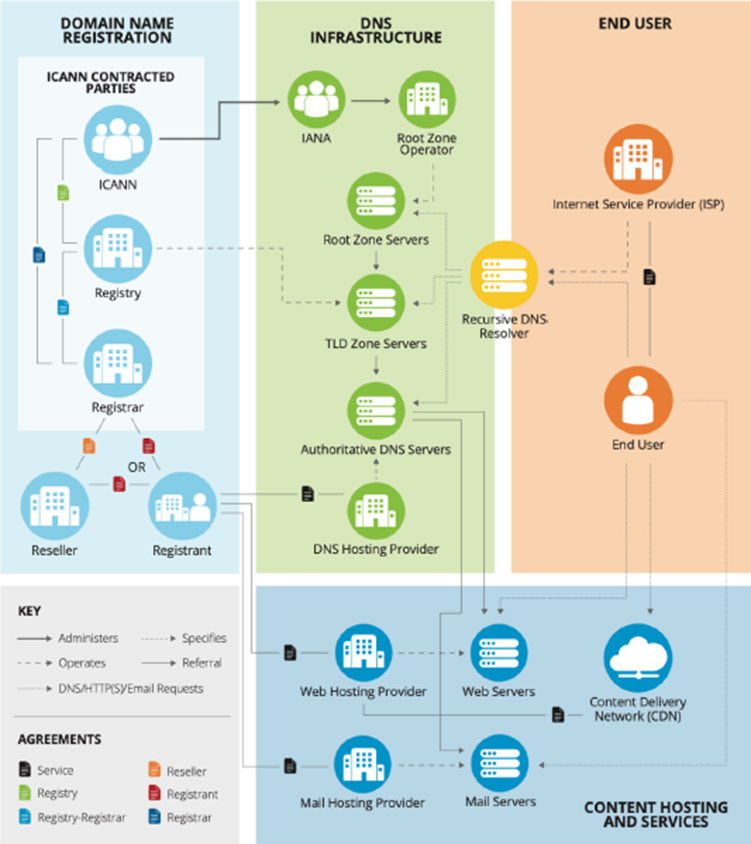
\includegraphics[width=1.0\linewidth]{background/DNSECO.png}
    \caption{DNS Ecosystem Contractually Related to ICANN (image
courtesy of Verisign and originally published in SSAC 115)}
    \label{fig:fig14}
\end{figure}
\clearpage

\section{Technological Advancements}

The mitigation of DNS abuse is increasingly influenced by the integration of artificial intelligence (AI) and machine learning technologies \cite{goethals2021enabling}. At the helm of this evolution are innovative tools like the iQ Domain Risk Score, which employs machine learning and string analytics to proactively detect potential domain abuses now of registration \cite{dnsabuseAI2023}. This tool aims to act as a mitigation measure by analysing domains against criteria indicative of malicious intent, thereby attempting to stop abuse before it even starts. Additionally, the field is witnessing a transformative shift in analysing abuse report evidence through the adoption of Large Language Models (LLMs), such as generative pre-trained transformers (GPTs). These models are highly adept at parsing and understanding complex data patterns that might be missed by human investigators, enhancing the efficiency and automation of DNS abuse mitigation efforts, and forming a more dynamic defence against cyber threats. However, this progress also highlights an emerging challenge: the potential for malicious entities to exploit AI technologies themselves \cite{halvorsenAI2023}.  Consequently, the intersection of AI and machine learning with DNS abuse mitigation not only heralds significant advancements in cybersecurity strategies but also emphasizes the need for vigilance to prevent these technologies from being used for harmful purposes. This pivotal moment in the fight against DNS abuse underscores the need for ongoing innovation and adaptation to effectively secure digital ecosystems.

\subsection{Role of AI and Machine Learning}

The introduction of AI and machine learning technologies into DNS abuse mitigation marks the beginning of an innovative era focused on the proactive detection and neutralisation of cyber threats \cite{tariq2023critical}.  This approach facilitates the rapid analysis of large datasets to uncover patterns indicative of malicious intent in DNS queries. For example, machine learning techniques have been highly effective in analysing DNS queries to classify domain names, significantly improving the detection of domains linked to malware \cite{LiMaliciousDomainDetection2020}. Furthermore, the application of neural network models, such as the Extreme Learning Machine (ELM), has achieved accuracy rates above 95\% in identifying malicious domains, demonstrating the transformative and predictive power of AI in combating cyber threats \cite{ZouDNSGraphMining2015}. Additionally, the technique of DNS graph mining has illuminated AI's potential within cybersecurity frameworks, with methodologies like belief propagation algorithms achieving high precision in identifying infected hosts and malicious domains. These examples underscore the vital role of AI and machine learning in bolstering DNS abuse, paving new avenues for early detection and swift mitigation of potential abuses. However, the complexity of AI models and the demand for transparency in their decision-making processes present ongoing challenges. Integrating AI into DNS abuse mitigation strategies improves security measures, but also requires careful attention to ethical considerations and the establishment of governance frameworks \cite{AntonakakisMalwareDomainsUpperDNS2011}. AI and machine learning can help improve DNS abuse mitigation, but experts need to fix problems by being clear. People are worried about understanding why complex systems make choices because of the "black-box" part. It is important to understand how AI models make certain decisions. This helps to build trust and ensures that people are responsible for them. There are difficulties in making things clear, such as needing to write down what data was used for training, telling others about the things that affect choices, and explaining how models change to face new risks. It is still hard to find the right balance between the complexity needed for good threat detection and the openness needed for blame.

In summary, leveraging AI and machine learning for DNS abuse mitigation signifies a transformative shift in cybersecurity practices. The strategic application of these technologies substantially strengthens the DNS system's defence against a wide array of cyber threats, marking a significant advancement in the ongoing battle against digital abuse.

\section{Case Studies and Real-World Applications}

In recent years, technology has become so widespread that we have witnessed an unmatched number and complexity of cyber threats. A significant vulnerability that can be exploited is the DNS domain name system, a critical part of the internet infrastructure that translates human-readable names into IP addresses \cite{kumari2021sac115}. 

\begin{enumerate} 
\item\textbf{ Case Study 1: XYZ Corporation }

In this case, the study completely analyses one specific company, XYZ Corporation, as an example of DNS abuse in the real-world environment and analyze all details through figures, graphs, and charts. This abuse of DNS took place as a prolonged campaign against XYZ Corporation, a multinational technology conglomerate \cite{mohammed2021network}. Attackers used weaknesses in the company's DNS infrastructure to perform various malicious activities, including domain hijacking, DNS tunneling, and DDoS attacks. A timeline graph was also prepared to see the scale of abuse and how attacks progressed with each event that occurred in the organisation, as shown in Figure \ref{fig:figureOne}.

\captionsetup{font= footnotesize}
\begin{figure}[H]
\centering
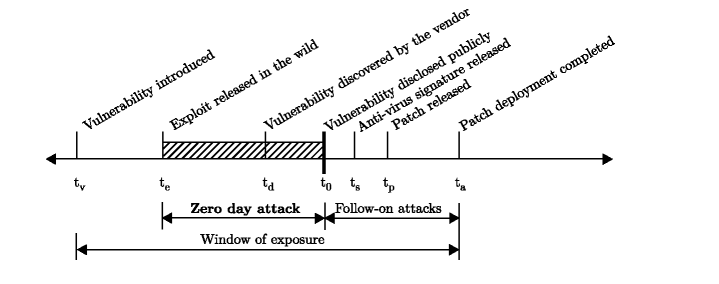
\includegraphics[width=0.9\textwidth]{background/XYZ1.png}
\caption{Timeline of DNS Abuse Attacks on XYZ Corporation}
\label{fig:figureOne}
\end{figure}

The relationship between this correlation raises questions about the attackers' understanding of the inner workings of the firm, as well as insider threats. A closer analysis of the DNS abuse types employed by such offenders revealed that domain hijacking was common \cite{bayer2022study}. Figure \ref{fig:figureTwo} shows how various DNS abuse techniques were used in the case of XYZ Corporation, and domain hijacking was significantly higher than all other combined methods.
\captionsetup{font= footnotesize}
\begin{figure}[H]
\centering
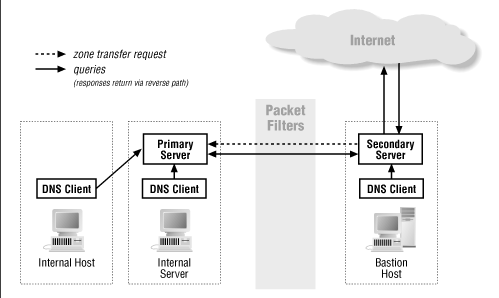
\includegraphics[width=0.8\textwidth]{background/XYZ2.png}
\caption{Distribution of DNS Abuse Techniques Against XYZ Corporation}
\label{fig:figureTwo}
\end{figure}

There is a domain hijacking technique where attackers may effectively take control over a company without authorisation; domain hijacking is one of the major threats to the organisations that are affected. The figure shows that strong security is key to preventing unauthorised access to domain registration accounts; favouring multi-factor authentication is the way to keep these attacks away \cite{paz2020cyber}. This case study sheds light on the subtleties of DNS abuse as it targeted XYZ Corporation, showing the importance of understanding and dealing with an unpredictable cyber threat environment. Figures, graphs, and graphs serve to illustrate safeguard attack procedures and give credence to the notion that an all-encompassing cybersecurity strategy is integral to mitigating DNS abuse in the digital landscape of the networked world of our day.


\item\textbf{ Case Study 2: OilRig DNS Tunneling Attack }

The case of OilRig reflects the use of custom DNS Tunneling protocols for command and control (C2) operations, thus making it dual use in nature, both in normal operation and on a fallback communication channel \cite{paloaltonetworks2021dnsattacks}.The xHunt campaign \cite{unit42_xhunt_2021} followed a similar trend of including Snugy backdoor implants in Middle Eastern government organization targets and keeping track of them using DNS tunneling for communication with its C2.  Which are examples that underscore the strategic use by adversaries of DNS tunneling techniques for stealthiness and resilience within the context of their operations  \cite{unit42_2021}.

\captionsetup{font= footnotesize}
\begin{figure}[H]
    \centering
    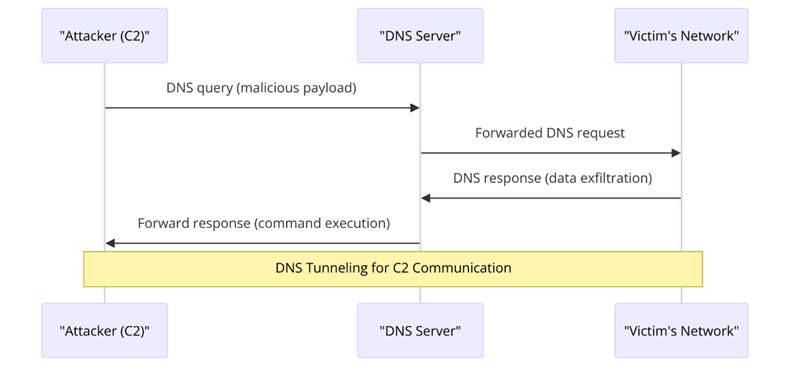
\includegraphics[width=0.8\linewidth]{background/DNSTuu.png}
    \caption{DNS tunneling communication between the attacker's command and control (C2) infrastructure and the victim's network}
    \label{fig:figTen}
\end{figure}



\item\textbf{ Case Study 3: SUNBURST Use of DGAs}

SUNBURST backdoor associated with the breach of the SolarWinds supply chain represents a case in which the use of DGAs is critical, if not only, to conceal communications and system details \cite{paloaltonetworks2021dnsattacks}. The SUNBURST backdoor applies the deep use of DNS manipulation for evasion purposes and subsequent attack stages by encoding basic system identifiers and the usage of DGAs for C2 check-ins \cite{unit42_solarstorm_2021}.

\captionsetup{font= footnotesize}
\begin{figure}[H] 
    \centering
    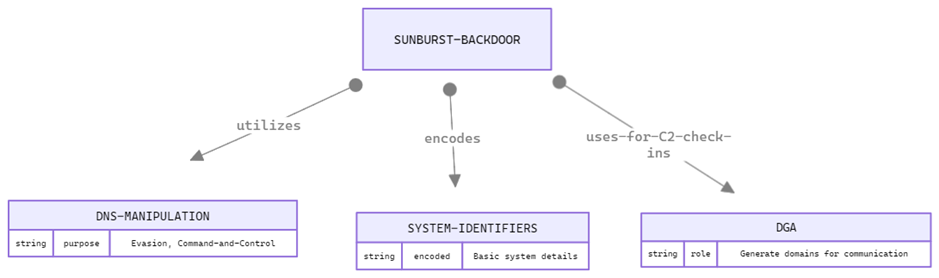
\includegraphics[width=0.8\linewidth]{background/SUNDNS.png}
    \caption{SUNBURST backdoor's utilization of DGAs and its associated components}
    \label{fig:figEleven}
\end{figure}

\item\textbf{ Case Study 4: Fast Flux Techniques}
The presence of several C2 domains related to the Smoke Loader malware family using Fast Flux techniques only further underscores the difficulties associated with the tracking and eradication of DNS-enabled threats. \cite{paloaltonetworks2021dnsattacks}.The major takeaway in the rapid rotation of IP addresses of this method points to the dynamism of strategies used in communications by malware, thus improving the means of defence by cybersecurity \cite{unit42_fastflux_2021}.

\captionsetup{font= footnotesize}
\begin{figure}[H]
    \centering
    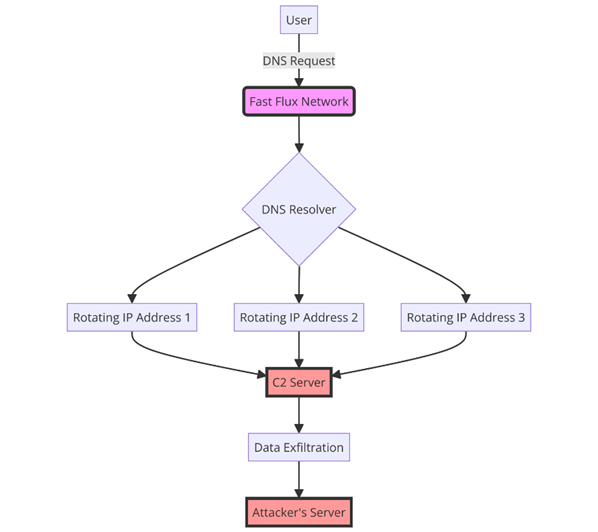
\includegraphics[width=0.8\linewidth]{background/FastFluDNS.png}
    \caption{The usage of Fast Flux techniques by the Smoke Loader malware family for dynamic C2 domain communications}
    \label{fig:figTweleve}
\end{figure}


\item\textbf{Case Study 5:  Malicious Newly Registered Domains (NRDs)}

The malicious NRDs opportunistically crafted in the milieu of the pandemic expose how threat actors leverage current events for engineering targeted attacks. \cite{paloaltonetworks2021dnsattacks} From domains that mirror COVID-19 information resources to those faking government relief programmes, the evolution of such attacks reflects a calculated approach to exploiting public interest and vulnerabilities  \cite{unit42_covid19_phishing_2021} .

\captionsetup{font= footnotesize}
\begin{figure}[H]
    \centering
    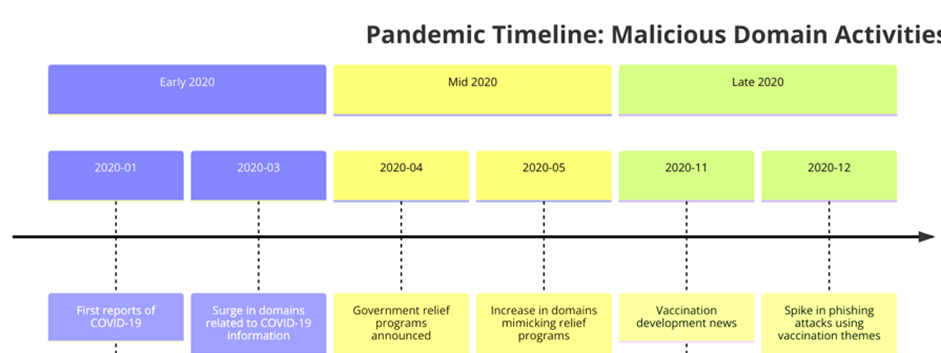
\includegraphics[width=0.8\linewidth]{background/PandemicTime.png}
    \caption{The usage of Fast Flux techniques by the Smoke Loader malware family for dynamic C2 domain communications.}
    \label{fig:figThirteen}
\end{figure}

\end{enumerate}

In the coronavirus pandemic, too, phishing attacks changed to initially targeting PPE and testing kits, then turning to government stimulus programs, and subsequently enlisting vaccine distribution. Several of them, in fact, employed sophisticated tools like MFA pretending as US Federal Trade Commission and brands such as Pfizer and BioNTech, to steal credentials. where it emphasized that there was a 530\% surge in vaccine-related phishing attempts and a 189\% hike in attacks on pharmacies and hospitals from December last year to February this year. Advice was given for individuals and organisations that include being cautious in email and website dealings, stepping up security awareness training, as well as adopting multi-factor authentication.

Since January 2020, a total of 69,950 COVID-19 related phishing URLs have been received, of which 33,447 are specifically dedicated to COVID-19. The data has been normalized in such a way that the peak of each topic is at 100\%. The results showed much steadier phishing when it came to topics such as pharmaceuticals and virtual meeting platforms (e.g., Zoom) with vaccines and testing showing sharper rises and falls in the attention of scammers.

\captionsetup{font= footnotesize}
\begin{figure}[H]
    \centering
    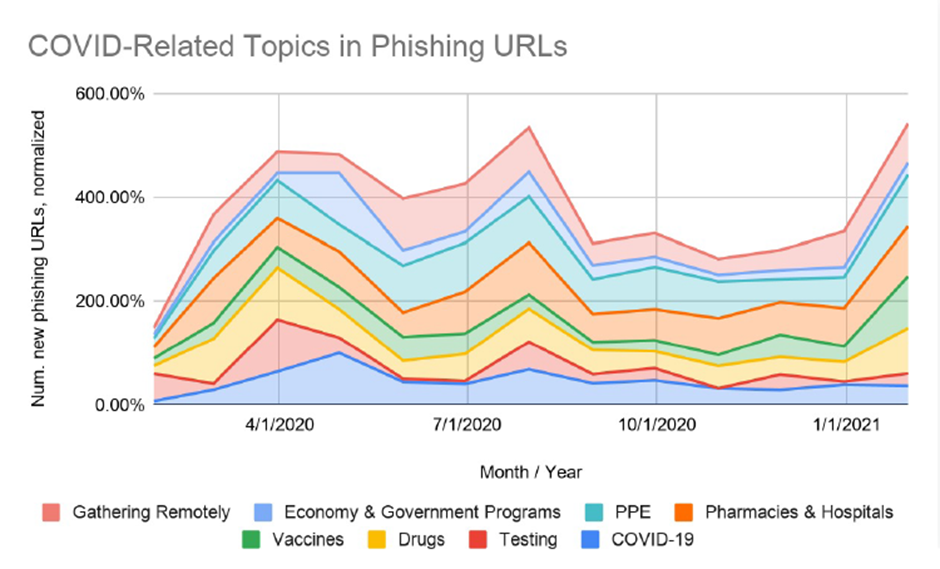
\includegraphics[width=0.8\linewidth]{background/CovidPhising.png}
    \caption{Development trends in the majority of COVID-19-related phishing content hosting sites during the period from January 2020 to February 2021.}
    \label{fig:figFourteen}
\end{figure}

It is evident to state that a major chunk of COVID-19-themed phishing pages targeted leading brands for phishing business credentials, such as Microsoft login, Webmail, and Outlook login. For example, about 23\% of these phishing URLs were posed as Microsoft login pages. This threat has particularly highlighted the shift towards remote work in the pandemic and, hence, magnified the relevancy of these attacks as one of the foremost methods to be undertaken by cybercriminals.


\captionsetup{font= footnotesize}
\begin{figure}[H]
    \centering
    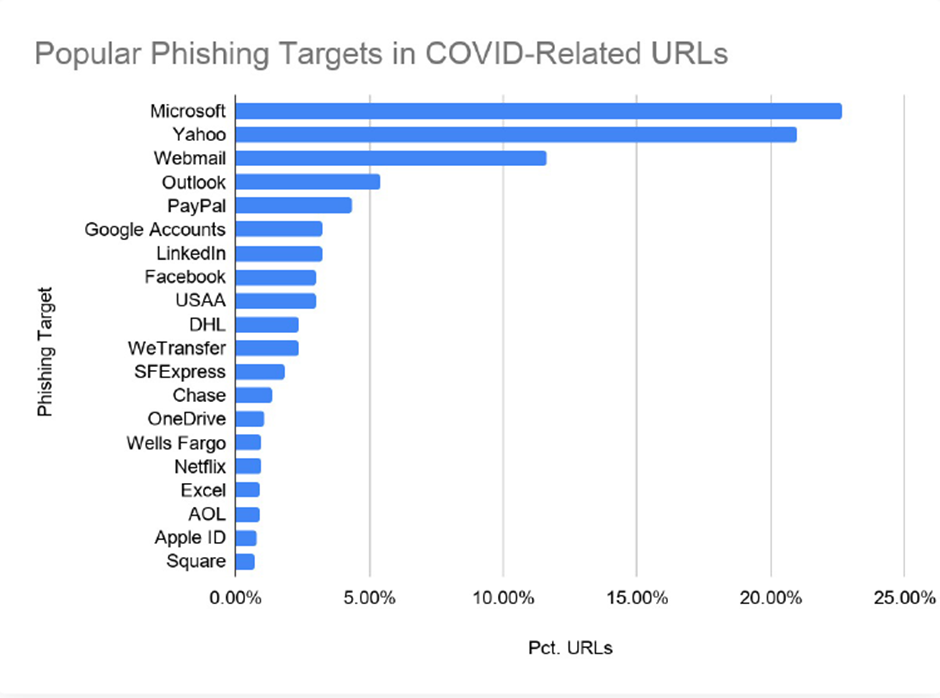
\includegraphics[width=0.8\linewidth]{background/TOPCOVIDURLS.png}
    \caption{Top spoofed websites in COVID-themed phishing attacks (global), where the percentage in each column is the percentage of phishing volume per site and category. }
    \label{fig:figFiveteen}
\end{figure}

This thus clearly indicates a situation whereby the attackers set up websites frequently for COVID-19 themed phishing attacks. Many of these phishing pages are found on sites created less than 32 days, meaning these sites are launched with specific purposes in view of these imminent attacks. The strategy allows attackers to customise their messages and URLs to the current pandemic trends, indicating the dynamism behind such cyber threats.

\captionsetup{font= footnotesize}
\begin{figure}[H]
    \centering
    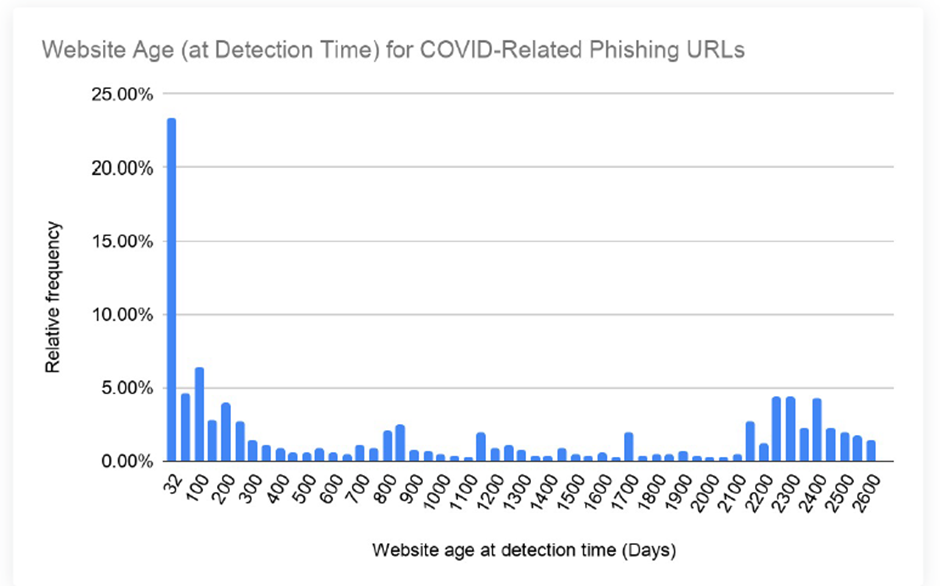
\includegraphics[width=0.8\linewidth]{background/AgeCovid.png}
    \caption{Statistic of lifespan distribution of COVID-19-related phishing content hosting sites when the sites are reported .}
    \label{fig:figSixteen}
\end{figure}


\section{Challenges and Future Directions}

Mitigating DNS abuse demands an immediate stop to the escalation and rapid evolution of cyber threats, underscoring the critical need for swift global cooperation and the implementation of advanced technology. The key challenge is to achieve a fine balance between reducing false positives and accurately identifying genuine threats, while simultaneously advancing beyond the limitations of outdated technologies \cite{pour2023comprehensive}. The future of this domain largely depends on researchers' ability to enhance technological solutions, particularly focusing on the improvement of AI algorithms for deeper analysis of DNS traffic patterns. This opens a promising pathway for the creation and application of locally developed tools, providing innovative strategies to strengthen DNS defences. The ability to navigate the complex landscape of DNS abuse will require stakeholders to be agile in responding to emerging threats and developing novel solutions. The collective push towards the evolution of technology and methodologies will play a pivotal role in shaping effective DNS abuse management strategies in the years ahead.


\subsection{Identification of Current Challenges}

Mitigating DNS abuse involves developing strategies that should be not only proactive but kept constantly up to date to handle the changing environment of cyber threats. The fluid nature of these threats means updating current protocols as well as developing new defence methods. With cybercriminals constantly revising their methods of capitalizing on the vulnerability of DNS, it has become imperative for the cybersecurity industry to continuously update its defence mechanisms \cite{bhattacharya2023dns}. Being a global phenomenon, the internet, and hence DNS abuse being transnational in character, there is no other alternative than international cooperation. The effectiveness of the DNS abuse management would be based on collaborative work across national borders, where experts in different geographical areas come together to share their knowledge and resources \cite{altulaihan2022cybersecurity}. Legal and regulatory framework varies in the several jurisdictions, thereby making it difficult to reach a consensus on the regulations, standards, and enforcement action. Another big challenge is that, to mitigate DNS abuse, the requirement for driving down both false positives and negatives is necessary. Balance must be established in such a way that rather strict measures may reduce user experience, while, at the same time, being liberal might bring less detection of malicious activities \cite{lyu2022survey}. The cybersecurity community must continue to advance its detection and response capabilities, due to the increasing levels of sophistication used by DNS abusers. This will keep the security and integrity of the DNS system in good shape, hence protecting this vital part of internet infrastructure.

\subsection{Discussion on Future Research Directions and Technologies}

When planning to mitigate the DNS abuse in the future, discussing new research ideas and upcoming technology is important. The constantly changing state of Internet threats requires us to continually create new things. This is so people can stay one step ahead of the bad people. Future work on DNS abuse needs to start by building better tools. These can help to address how bad guys on the Internet keep changing their tricks \cite{bovenzi2023blockchain}. This means that we need to look at more complex AI and machine learning tools that can understand the details of web traffic which will make the results more accurate and stop wrong signals from being sent. Moreover, there is a rising need to use blockchain tech to make domain registration safer and stop any bad or harmful changes, as it provides decentralised domain name resolution unlike traditional DNS systems, which rely on a central authority to resolve domain names, a Blockchain DNS operates on a network of distributed nodes in which each node has a copy of the entire blockchain ledger, so it can independently verify and resolve domain name requests, which not only makes the system more resilient to attacks but also prevents censorship and control by a single entity. \cite{FinanceStrategists2023BlockchainDNS}.  People should have easy methods to report DNS abuse. This will make sure everyone knows about dangers \cite{gu2021iot}. Working together in the world is very important because computer dangers go beyond borders. 


\section{Conclusion}

DNS abuse continues to be a big issue. Present plans, while sometimes useful, require constant adjustment and getting better. It's key to have solutions for fixing issues available. This helps to build trust and work well with those involved. Abusing DNS in new ways brings fresh issues that require clever solutions. AI and machine learning can help find things, but we need to show how they work better so that people can keep bad people under control. Learning from real-life situations teaches us a lot about good and bad ways of being open. This helps us create the best methods for our business. There are still issues with showing and stopping DNS abuse while trying to find new ways to mitigate this DNS abuse. People need to continue learning and working as a team. People should focus on better technology, joining forces with other nations, and using common methods of sharing information in the future. As the internet changes, we must stay active and work together to stay ahead of bad people who want to hurt us. 

\section{Summary of Findings}

The study on DNS abuse looked at current ways, checked new trends, talked about tech advancements, and explored real examples in life. The search for ways in the plans to mitigate DNS abuse showed the value of clear communication and honesty in building trust with the community. People are finding new ways to abuse the DNS system. Researchers have to keep making new things, so they don't get caught by changing dangers. Improvements in technology, especially with artificial intelligence and learning machines, showed how automation can make it easier to spot dangers. But it also made things harder to understand, and this needs careful attention. Examples from real life showed what did and did not work in making DNS abuse clearer. These provided essential advice for the business. Issues with making things clear and stopping wrong actions were found. This shows how important it is to continue learning and working with others. In the future, discussing issues and future plans will show the need for creative studies, help from other nations, and common ways to share information. 





















